\documentclass[12pt]{article}
\usepackage{graphicx} % Required for inserting images
\usepackage[letter,margin=1in]{geometry} % Adjust margins if needed
\usepackage[utf8]{inputenc}
\usepackage{hyperref}
\usepackage{url}
\usepackage{wrapfig}
\usepackage{titlesec}
\titlespacing*{\section}{0pt}{0\baselineskip}{0\baselineskip}
\titlespacing*{\subsection}{0pt}{0\baselineskip}{0\baselineskip}

\usepackage[
backend=biber,
style=nature,
]{biblatex}
\addbibresource{references.bib}

\begin{document}

\begin{center}
    \Large{\textbf{Grant Proposal: A Geospatial and Temporal Analysis of Lead Pollution From Piston Aircrafts Near Kelowna International Airport Using AES with ADS-B Data}}\\
    \vspace{1cm}
    \large{Wenqi Guo}\\
    \vspace{0.5cm}
    \large{UBCO CHEM 434 Assignment}\\
    \vspace{0.5cm}
    \textit{Project Duration: 2 months}\\
    \vspace{0.5cm}
    \textit{Funding Agency: UBC and Interior Health}\\
    \vspace{0.5cm}
    \textbf{Amount Required: \$1000}\\
    \vspace{1cm}
    \vspace{1cm}
    \today
\end{center}
\newpage

\section{Introduction and Background}
Lead has been known as a type of toxin and there is no known safe amount of lead: even a small amount of lead could lead to health issues, such as decreased IQ in children, high blood pressure, cardiovascular problems, and kidney damage. \cite{world_health_organization_lead_2023} Although leaded gasoline has been banned for on-road vehicles in the world, it is still used in many piston-engine powered small general aviation aircraft as 100LL (100 Low Lead), which contain tetraethyllead (TEL) and has a lead concentration of about 0.56g/L. 
\cite{noauthor_safety_2021} A past study has shown that the soil lead levels around airports in Oklahoma are not higher than the level of concern, but it did suggest long-term monitoring for soil lead levels. \cite{mccumber_geospatial_2017} More importantly, many other previous studies have shown that children near general aviation airports have elevated blood lead levels (BLL). \cite{miranda_geospatial_2011} \cite{zahran_leaded_2023} \cite{mills_lead_2022} \cite{zahran_effect_2017} Additionally, the United States Environmental Protection Agency has very recently issued a determination that lead-emission from position engine aircraft cause or contribute to air pollution, giving reasonable anticipation that it may endanger public health and welfare. \cite{us_epa_epa_2023}


 However, it is not feasible to do blood or soil lead levels around every general aviation airport. A media report collected the Automatic Dependent Surveillance-Broadcast (ADS-B) data, which provides the tracking data of an aircraft's real-time information like location and altitude, and used the flight path and altitude to estimate lead exposure levels for the surrounding area. They mapped the flight frequency where the plane altitudes were lower than 10,000 feet. \cite{noauthor_you_2022} However, this is a semi-quantitative analysis: it might be reasonably accurate in estimating relative lead contamination for different areas, but it cannot give a numeric result of the amount of lead exposure and thus it cannot estimate the actual risk from lead exposure. 

Kelowna International Airport (CYLW) serves both commercial and general aviation airplanes. Although its location is remote from Kelowna downtown, it is not distanced from some residential neighbourhoods such as Glenmore Highland and Rutland (about 5km and 4km to the end of CYLW runway, respectively). Given Kelowna's growing population and potential growth in residential areas, the close proximity of the airport is a valid public health concern. Additionally, the end of its runway is only about 1km from the University of British Columbia Okanagan Campus (UBCO), which is a growing educational and research institution with many students and staff, and there are about 2000 students who live on campus\footnote{\url{https://ok.ubc.ca/about/facts-and-figures/}}. This also raised concerns about possible lead contamination around the campus.

Another student project from UBCO analyzed the soil sample around CYLW and found that the highest soil lead level is $11.55\pm 1.38$ mg/Kg, in Lake Country, which does not reach the level of concern. \cite{harrison_lead_nodate} (Usually soil lead levels between 10-50 ppm do not have detrimental health effects.) \cite{noauthor_lead_nodate} Although their study does consider the flight directions (flights usually take off on the south side and land on the north side), they did not consider the effects of wind direction on lead distribution: although flights are taking off southbound, they usually take off against the wind, meaning the wind is blowing toward the north side and could carry the lead particles to the north side of the airport. \cite{harrison_lead_nodate} Additionally, soil samples are less time-sensitive when responding to aviation activities and might not be able to attribute the cause of lead in soil compared to air samples. 

In this study, we will collect the topsoil samples and air samples around the airport and analyze their lead level using ICP-AES. We will also collect the ADS-B data from the aircraft near CYLW from ADSB Exchange\cite{adsbexchange}. We will then analyze the geospatial and temporal correlation between the ADS-B data and lead level and determine if the air lead level is higher under the flight paths or when flight activities are more frequent and if soil and air lead levels on the downwind side and underneath of the flightpath are higher than the upwind side. 
\setlength\intextsep{-2pt}
\begin{wrapfigure}{r}[1cm]{0.3\textwidth}
  \begin{center}
    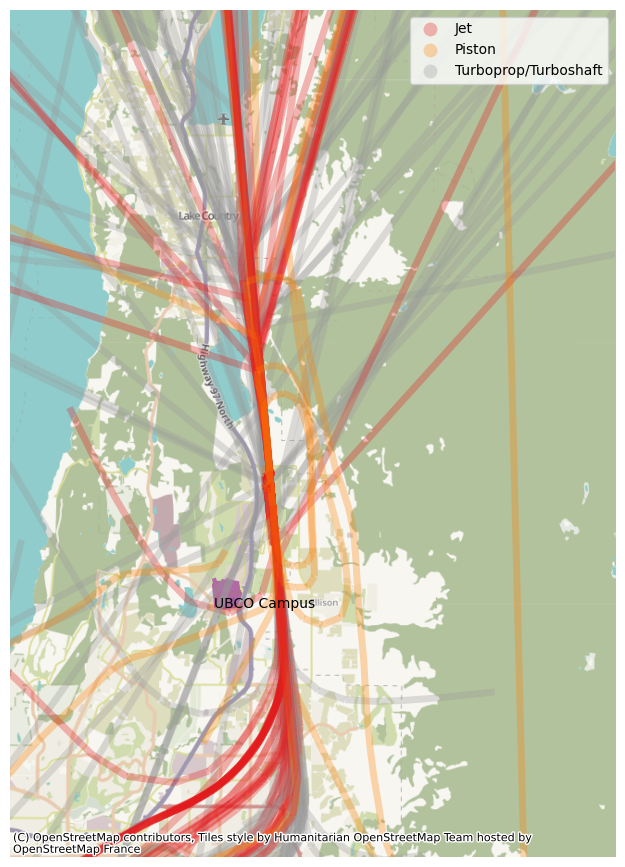
\includegraphics[width=0.3\textwidth]{map.png} \\
  \caption{\small{Sample Map of Air Trafic Below 5000 ft Captured around CYLW on Nov 15, 2023}}
      \label{fig:map}\\

          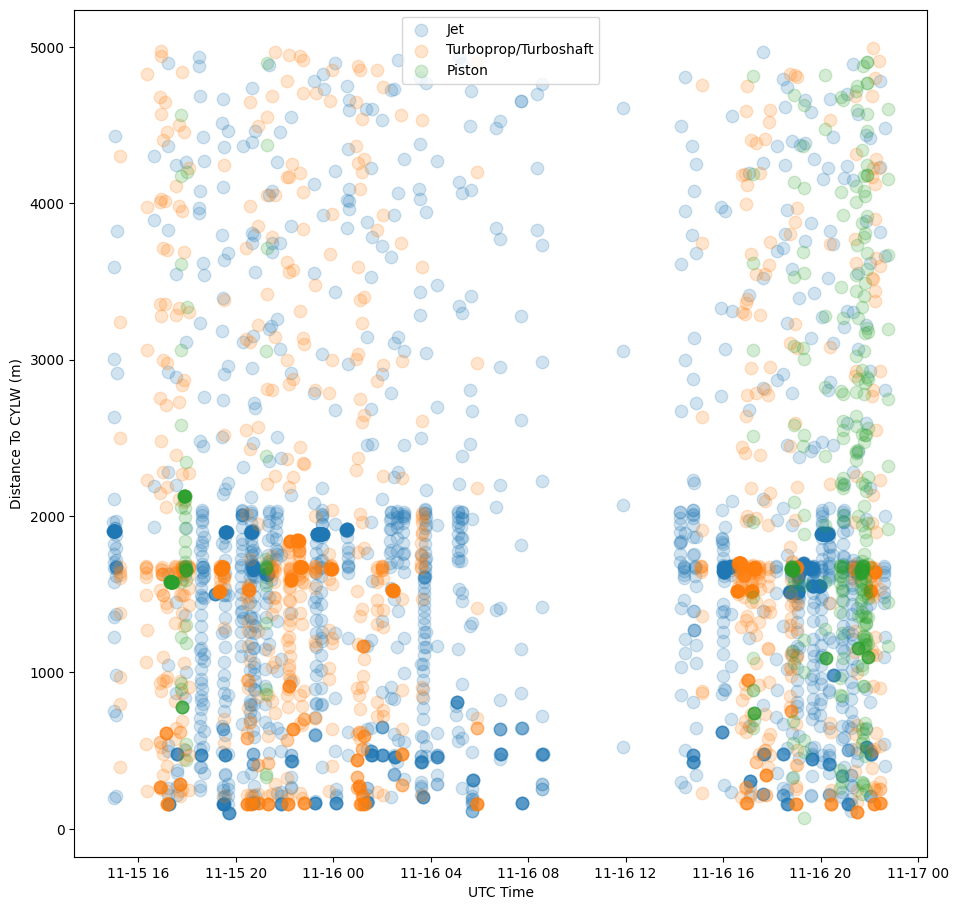
\includegraphics[width=0.3\textwidth]{time.png} \\
  \caption{\small{Sample Air Trafic Plot Across Time and Distance}}
      \label{fig:time}
  \end{center}
\vspace{-20pt}
\end{wrapfigure}
\section{Statement of Purpose}


Although leaded gasoline has been banned worldwide for on-road vehicles, it is still commonly used for small piston-engine powered general aviation (GA) aircraft. (The fuel commercial jets use is not leaded.) Previous study has shown that children near GA airports have elevated blood lead level.\cite{miranda_geospatial_2011} \cite{zahran_leaded_2023} \cite{mills_lead_2022} \cite{zahran_effect_2017} Kelowna International Airport is a busy airport that serves both GA and commercial aircraft. With the growing population in Kelowna and the UBCO campus, the lead emission from GA aircraft in this area is a public health concern. In this study, we aim to analyze the topsoil and air lead levels around the Kelowna International Airport using ICP-AES (an elemental analysis technique) to determine if there is a lead exposure concern for people living nearby and students and staff of UBCO. We will also incorporate it with the ADS-B data near the airport, which will provide the location and altitude information of the aircraft. This allows us to find the geospatial and temporal relations between the aircraft's activities and topsoil and air lead levels. The correlation could help us better understand how aviation activities affect soil lead levels and can help us build a model to predict soil lead levels using ADS-B data, providing an affordable alternative method for estimating soil lead levels compared to chemical analysis.
\section{Methods}
\subsection{Data Collection}\footnote{Parts of this section are down as a demo and shown in \textbf{Figure} \ref{fig:map} \ref{fig:time}}
There are many ASD-B data providers on the market. In this study, we will use the Application Programming Interface (API) from ADSBExchange \cite{adsbexchange} to capture such information. We will capture the ADS-B data in 8 one-week time spans. The data capturing starts at 7 am on the first day of the week and ends at 10 pm on the last day of the week. During the capture, we will request the API such that all the aircraft are within 50 nautical miles (about 92.6km) and we will log the data every 2 seconds. The data we are interested in are altitude, location (latitude and longitude), ICAO type designator (used to determine the engine type), vertical speed, and ground speed (used to predict the engine power and thus estimate the fuel consumption). At the same time, wind direction data around CYLW is also captured at the rate of once per minute using a real-time weather data provider Open Weather Map. 

After capturing the data, we will filter out flights with altitudes higher than 5000 feet, and then we will look up the engine type of the aircraft using the ICAO type designator from ADSBExchange in the Aircraft Characteristics database \cite{faa}. For flight types that are not in the database, we will manually look up their engine and label them. We will code a Python script\footnote{The code used in the demo process to process the data could be found in \url{https://github.com/weathon/chem434/}} to use GeoPandas and Open Street Map \cite{OpenStreetMap} to overlay the flight paths onto a map. (A sample map was shown in \textbf{Figure} \ref{fig:map}) Additionally, we will also visualize different engine types across the dimensions of time and distance to the airport. This will be helpful for the temporal analysis of the relation between air traffic and air lead level. An example plot is shown in \textbf{Figure} \ref{fig:time}.

% something missing

This data will provide general information about the air traffic. However, not all aircraft broadcast their ADS information, especially small aircraft. At the same time, not all piston engines use 100LL. They could use unleaded gas or jet fuel. Thus, there might be some error between information from ADS-B and real leaded-gas-powered aircraft traffic. 

\subsection{Sample Collection And Analysis}
Since usually the airways are fixed and the flight paths would not deviate far from time, we will decide the sampling locations based on the flight path collected in the first week. We will collect the top soil sample at locations at the busiest flight paths near the UBCO campus and 2 locations upwind and downwind of the location. At each location, we will collect 3 topsoil samples. The location where the first sample was taken will be recorded and the following sampling location should be as close to the first location as possible. 

After the soil sample is collected, it will be digested with heat and acid with one of the methods in  \cite{moor_determination_2001}. Since handling hydrofluoric acid is dangerous, we decided to use the method with aqua regia, despite it having worse accuracy. The soil will be dried at 105 degrees for 3h, and then 0.5g of each sample will be weighed and placed in a beaker. It will be heated with 12mL of aqua regia for 45 min, then evaporated to almost dryness. 2.5mL of concentrated hydrochloric acid and 2.5 mL of H$_2$O$_2$ will be then added and the solution was accurately diluted to 50mL with water. \cite{moor_determination_2001} Then the solution will be tested using ICP-AES. We average the results for samples from the same location. 

\begin{wraptable}{r}{0.5\textwidth}
    \centering
    \begin{tabular}[0.3\textwidth]{|c|c|c|}
    \hline
    Step & Digestion Reagent & Rinsing Reagent \\ \hline
    1 & 50mL of aqua regia & 10\% HNO_{3} \\ \hline
    2 & Concentrated HNO_{3} & 10\% HNO_{3} \\ \hline 
    \end{tabular}
    \caption{\small{Reagents used to digest and rinse the sample according to \cite{gharaibeh_determination_2010}}}
    \label{tab:steps}
    \vspace{0.2cm}
\end{wraptable}

For air samples, we will use methods that are similar to \cite{gharaibeh_determination_2010} and \cite{vijayanand_assessment_2008}. Three high-volume air samplers will be respectively placed in an upwind location of the flight path, underneath the flight path, and in a downwind direction of the flight path. They will collect the air sample at the same time. New filters will be replaced every 2 hours. The whole collection will last about 8 hours and at least 5 position aircraft flyby occurs. 


After the air sample is collected, we will use methods in \cite{gharaibeh_determination_2010} to digest the samples. A portion of each filter will be cut down into small pieces and placed in a beaker. Three digestion and rinsing will be applied to the sample. Reagents in each step are shown in \textbf{Table} \ref{tab:steps}. After each time the digestion reagent is added, the beaker will be covered and heated to 140$^{\circ}$C to near dryness. And the sample will be filtered and the beaker will be rinsed. After the second digestion, the sample will be heated again to near dryness, and 50mL of 10\% HNO$_{3}$ will be added to cool the sample down; then the solution will be diluted to 100mL using 10\% HNO$_{3}$. \cite{gharaibeh_determination_2010}


Then the lead concentration of the sample will be determined by ICP-AES. Unlike in \cite{gharaibeh_determination_2010}, we will only collect the air sample in 2h spans not 24h spans, and we need to compare the difference (which might be small) between samples, we need to use a method with higher accuracy and sensitive. Thus, we chose ICP-AES instead of AAS. Similar to \cite{gharaibeh_determination_2010}, we will also repeat each sample with 3 runs, and an unused air filter will also be included (using the same digestion method above) as the blank sample. 


\subsection{Data Analysis}
After all the data (ADS-B, wind direction history, and ICP-AES result) are collected, we will compare the lead concentration between different locations and across different times and perform statical tests to determine if aviation activities will increase the lead concentration in soil and air, and if being downwind of the flight path will increase the lead concentration. 
\section{Schedule}
\begin{center}
\begin{tabular}{|c|c|c|}
 \hline
 \textbf{Step} & \textbf{Begin Date} & \textbf{End Date} \\
 \hline \hline
Code for collection of ADS-B data & Nov 28, 2023 & Dec 1, 2023 \\
\hline
First Week ADS-B data collection & Dec 1, 2023 & Dec 7, 2023 \\
\hline
First Dirt Sample Collection & Dec 7 2023 & Dec 7, 2023 \\
\hline
Air Sample Collection & Dec 7 2023 & Dec 7, 2023 \\
\hline
First batch of samples lab work & Dec 7, 2023 & Dec 8, 2023 \\ 
\hline
Second Week ADS-B data collection & Dec 8, 2023 & Dec 14, 2023 \\
\hline
First batch of samples lab work & Dec 14, 2023 & Dec 15, 2023 \\ 
\hline
Repeat for 8 weeks & Dec 15, 2023 & Jan 29, 2024\\
\hline
All data processing and finishing the project& Feb 1, 2024 & Feb 28, 2024\\
\hline
\end{tabular}
\end{center}
\section{Conclusions}
In this study, we will try to 
\section{Budget and Justification}
\begin{itemize}
    \item API Data Collection Cost: \$350. This cost is used to log flight and weather data. Since we will capture the flight data once every 2 seconds, we will capture 2,419,200 entries of data. Additionally, since the data will be used for research purposes, the personal-use API endpoint from ADSBExchange cannot be used and we need the commercial endpoint. The estimated cost of the API is about \$200. For the weather data, we will capture 40,320 entries per month. Open Weather Map allows 1,000 free requests and charges 0.0015 USD for every additional request. This brings the cost to 60.33 USD per month or 120.66 USD for the whole study. These data is necessary for the analysis of the correlation between flight activities and wind direction with lead concentrations in topsoil and air samples. 
    \item ICP-AES Cost: 
\end{itemize}

\newpage
\printbibliography
\end{document}
